%\documentclass[aspectratio=169]
\documentclass[aspectratio=169,xcolor=dvipsnames]{beamer}
%\usetheme{Copenhagen}
\usetheme{boxes}
\setbeamertemplate{navigation symbols}{}
\setbeamertemplate{footline}[frame number]
%\setbeamertemplate{footline}{}
\usecolortheme{dove}   %[named=black]
\usepackage{appendixnumberbeamer}
\usepackage[utf8]{inputenc}

\usepackage{graphicx}         
\graphicspath{ {./Pictures/} }
\usepackage{amsmath}
\usepackage{amsfonts}
\usepackage{amssymb}
\usepackage{amsthm}
\usepackage{mathtools}
\usepackage{commath}
\usepackage{multimedia}
\usepackage{subcaption}
\usepackage[autolanguage,nosepfour]{numprint}
\usepackage{media9}
\usepackage{dashrule}
\addmediapath{Animations/}
\newcommand{\Sta}{y}
\newcommand{\Adj}{p}
\newcommand{\Con}{u}
\begin{document}


\begin{frame}

		\begin{figure}
			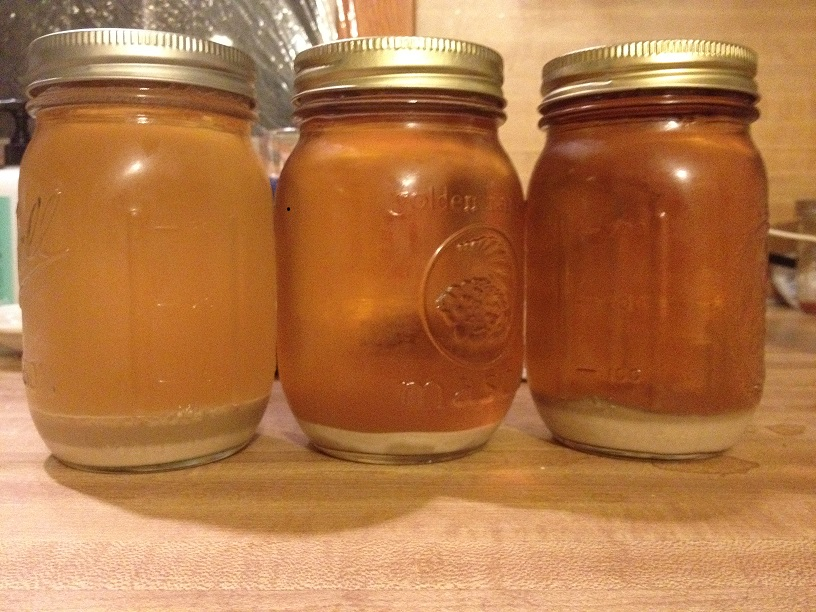
\includegraphics[width=5cm]{beer.png}
			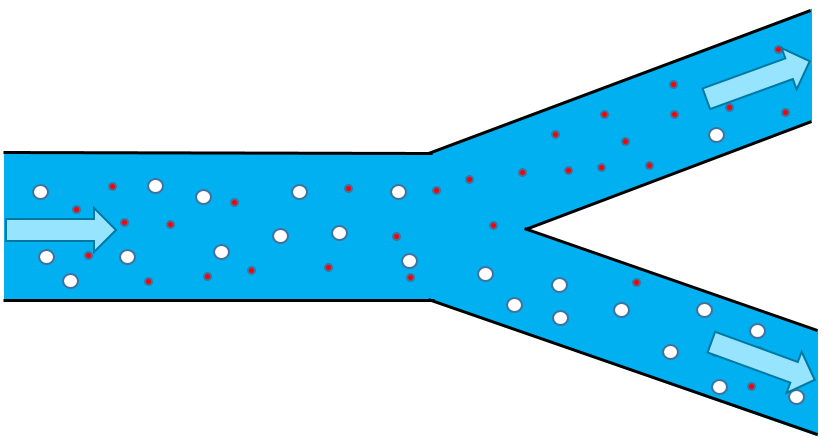
\includegraphics[width=7cm]{Microfilter.png}
			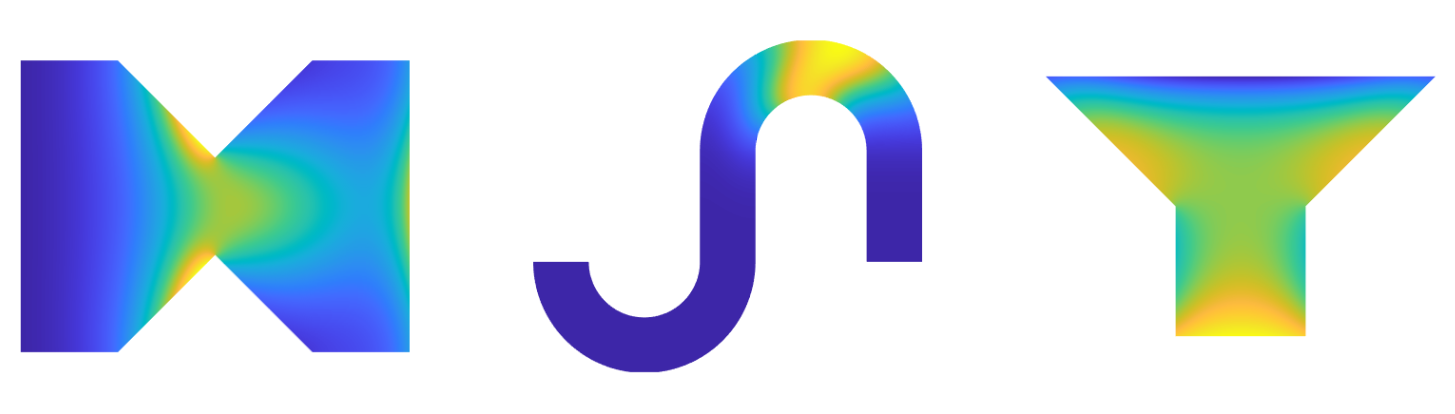
\includegraphics[width=12cm]{Future.png}
		\end{figure}
		
\end{frame}


\begin{frame}
	\frametitle{PDE-Constrained Optimization}
	\framesubtitle{A simple model}
		\begin{columns}
		\column{0.6 \linewidth}
			\begin{align*}
			&\min_{\rho,f} \quad \frac{1}{2}\norm{\rho- \widehat{\rho}}_{L_2(\Sigma)}^2 + 	\frac{\beta}{2} \norm{f}_{L_2(\Sigma)}^2\\
			\\ 
			&\text{subject to:}
			\\
			& \partial_t \rho = \nabla^2 \rho + f \ \qquad \text{  in    }\ \ \Sigma := 	(0,T) \times \Omega  \\
			\\
			&\text{BC } \text{and IC:}\\
			&\frac{\partial \rho}{\partial n}  = 0 \quad \ \ \qquad \qquad \text{on   } 	\partial \Sigma := (0,T) \times \partial \Omega  \\
			&\rho(0,\vec{x}) = \rho_0(\vec{x})
			\end{align*}
		\column{0.4\linewidth}
		\vspace{-0.8cm}
		\begin{figure}
			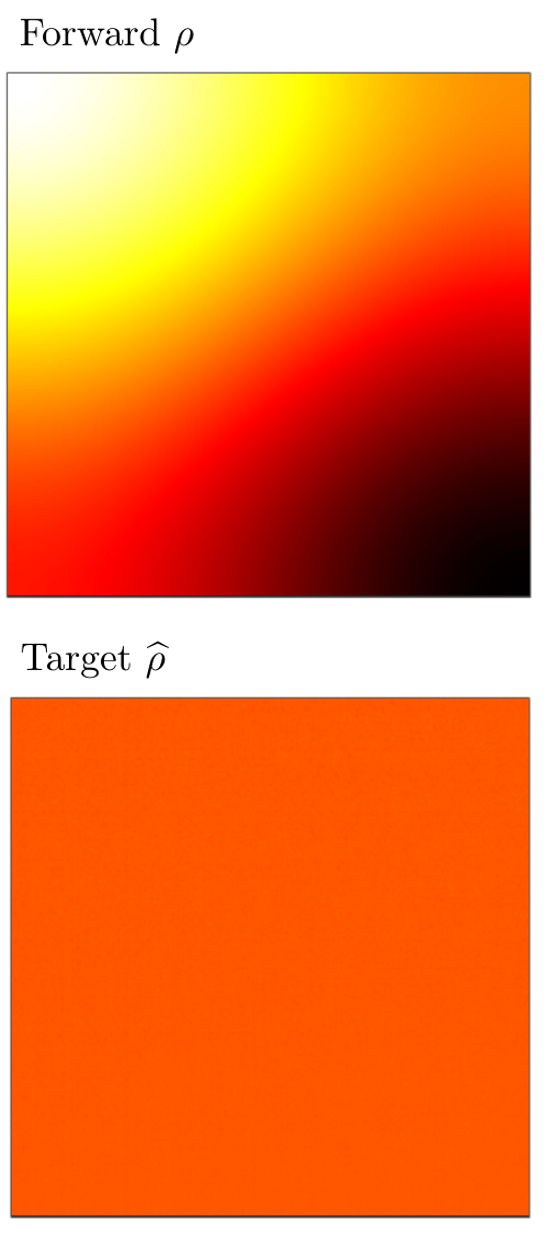
\includegraphics[width=3.2cm]{heat.png}
		\end{figure}
		\end{columns}
\end{frame}

\begin{frame}
	\frametitle{PDE-Constrained Optimization}
		\framesubtitle{Deriving (first-order) optimality conditions}
	Define the Lagrangian $\mathcal{L}$:
	\begin{align*}
		\mathcal{L}(\rho, f,q)=& \frac{1}{2}\norm{\rho- \widehat{\rho}}_{L_2(\Sigma)}^2 + \frac{\beta}{2} \norm{f}_{L_2(\Sigma)}^2- \int_\Sigma q \bigg( \partial_t \rho - \nabla^2 \rho  - f \bigg) d\vec{x} dt - \int_{\partial \Sigma} q \frac{\partial \rho}{\partial n}   d\vec{x} dt.\\
	\end{align*}
	Compute directional derivatives and set equal to zero:
	\vspace{0.1cm}
	\begin{align*}
		\mathcal{L}_q (\rho^*, f^*,q) h&= 0, \quad
		\mathcal{L}_\rho (\rho^*, f^*,q) h= 0, \quad
		\mathcal{L}_f (\rho^*, f^*,q) h= 0.
	\end{align*}
\end{frame}
\begin{frame}
	\frametitle{PDE-Constrained Optimization}
	\framesubtitle{Deriving (first-order) optimality conditions}
	\vspace{0.2 cm}
	Define the Lagrangian $\mathcal{L}$:
	\begin{align*}
		\mathcal{L}(\rho, f,q)=& \frac{1}{2}\int_\Sigma \left(\rho- \widehat{\rho}\right)^2 d \vec x dt + \frac{\beta}{2} \int_\Sigma f^2 d \vec x dt - \int_\Sigma q \bigg(\textcolor{PineGreen}{ \partial_t \rho - \nabla^2 \rho  - f} \bigg) d\vec{x} dt \qquad \qquad\\
		&- \int_{\partial \Sigma} q \textcolor{magenta}{\frac{\partial \rho}{\partial n} }  d\vec{x} dt.
	\end{align*}
	Computing  $\mathcal{L}_q (\rho^*, f^*,q)h = 0$ results in the forward problem:
	\vspace{0.1cm}
	\begin{align*}
		\textcolor{PineGreen}{\partial_t \rho } \ & \textcolor{PineGreen}{ = \nabla^2 \rho + f} \ \qquad \text{  in    }\ \ \Sigma \phantom{vhfoijoihewrbgjkngmcojrpf      hfhioewjgpfinioer nnf}\\
		\textcolor{magenta}{\frac{\partial \rho}{\partial n}} \ & \textcolor{magenta}{ = 0} \quad \ \ \qquad \qquad \text{on   } \partial \Sigma   \\
		\rho(0,\vec{x}) &= \rho_0(\vec{x})
	\end{align*}
\end{frame}

\begin{frame}
	\frametitle{PDE-Constrained Optimization}
	\framesubtitle{Deriving (first-order) optimality conditions}
	\vspace{0.3 cm}
	Define the Lagrangian $\mathcal{L}$:
	\begin{align*}
		\mathcal{L}(\rho, f,q)=& \frac{1}{2}\int_\Sigma \textcolor{magenta}{ \left(\rho- \widehat{\rho}\right)^2} d \vec x dt + \frac{\beta}{2} \int_\Sigma f^2 d \vec x dt - \int_\Sigma q \bigg( \textcolor{PineGreen}{\partial_t \rho} - \textcolor{CornflowerBlue}{ \nabla^2 \rho}  - f \bigg) d\vec{x} dt \qquad \qquad\\
		&- \int_{\partial \Sigma} q \frac{\partial \rho}{\partial n}   d\vec{x} dt.
	\end{align*}
	Computing  $\mathcal{L}_\rho (\rho^*, f^*,q)h$:
	\begin{align*}
		\mathcal{L}_\rho (\rho^*, f^*,q)h = & \int_\Omega\left( \textcolor{PineGreen}{q(T) h(T) - q(0) h(0)}\right)d \vec x  - \int_\Sigma \left(\textcolor{magenta}{ h(-\rho + \widehat \rho)}  - \textcolor{PineGreen}{h \partial_t q} - \textcolor{CornflowerBlue}{ h\nabla^2 q}  \right) d\vec{x} dt \\
		&-\int_{\partial \Sigma} \left( q \frac{\partial h}{\partial n}  \textcolor{CornflowerBlue}{- q \frac{\partial h}{\partial n} + h \frac{\partial q}{\partial n} } \right) d\vec{x} dt. \\
	\end{align*}
\end{frame}
\begin{frame}
	\frametitle{PDE-Constrained Optimization}
	\framesubtitle{Deriving (first-order) optimality conditions}
	Computing  $\mathcal{L}_\rho (\rho^*, f^*,q)h = 0$:
	\begin{align*}
		\mathcal{L}_\rho (\rho^*, f^*,q)h = & \int_\Omega q(T) h(T) d \vec x  - \int_\Sigma h \left(-\rho + \widehat \rho  - \partial_t q -  \nabla^2 q  \right) d\vec{x} dt - \int_{\partial \Sigma}  h \frac{\partial q}{\partial n} d\vec{x} dt = 0.\\
	\end{align*}
Adjoint equation:
\begin{align*}
	  \partial_t q &=  -  \nabla^2 q -\rho + \widehat \rho  \ \quad \text{in} \quad \Sigma \qquad \qquad\qquad\qquad\qquad\qquad\qquad\qquad\\
	  \frac{\partial q}{\partial n} &= 0 \qquad\qquad\quad\quad \quad \text{on} \quad \partial \Sigma\\
	  q(T, \vec x) &= 0
\end{align*}
\end{frame}

\begin{frame}
	\frametitle{PDE-Constrained Optimization}
	\framesubtitle{Deriving (first-order) optimality conditions}
	\vspace{0.2 cm}
	Define the Lagrangian $\mathcal{L}$:
	\begin{align*}
		\mathcal{L}(\rho, f,q)=& \frac{1}{2}\int_\Sigma \left(\rho- \widehat{\rho}\right)^2 d \vec x dt + \frac{\beta}{2} \int_\Sigma \textcolor{PineGreen}{f^2} d \vec x dt - \int_\Sigma q \bigg( \partial_t \rho - \nabla^2 \rho  - \textcolor{magenta}{f} \bigg) d\vec{x} dt \\
		&- \int_{\partial \Sigma} q \frac{\partial \rho}{\partial n}   d\vec{x} dt.
	\end{align*}
	Computing  $\mathcal{L}_f (\rho^*, f^*,q)h = 0$:
	\begin{align*}
		\mathcal{L}_f (\rho^*, f^*,q)h = & \int_\Sigma h \left(\textcolor{PineGreen}{\beta f} + \textcolor{magenta}{q} \right) d\vec{x} dt = 0.\qquad\qquad\qquad\qquad\qquad\qquad\qquad\qquad\qquad
	\end{align*}
	Gradient equation:
	\begin{align*}
		f = -\frac{1}{\beta}q. \qquad\qquad\qquad\qquad\qquad\qquad\qquad\qquad\qquad\qquad
	\end{align*}
\end{frame}
\begin{frame}
	\frametitle{PDE-Constrained Optimization}
	\framesubtitle{The (first-order) optimality system}
	
	\begin{align*}
		\partial_t \rho &= \nabla^2 \rho + \textcolor{blue}{f}  \\
		\partial_t q &=  -  \nabla^2 q - \textcolor{ForestGreen}{\rho} + \widehat \rho 
		\phantom{ngodshornvnien fjpisj wfseij gvjepi vwe  bfkdienwpiemf feq}\\
		\textcolor{blue}{f} &= - \frac{1}{\beta}\textcolor{red}{q}\\
		\\
		\frac{\partial \rho}{\partial n} &= 0, \qquad \rho(0,\vec{x})=\rho_0(\vec{x}),\\
		\frac{\partial q}{\partial n} &= 0, \qquad q(T,\vec{x})= 0.
	\end{align*}
\end{frame}
\begin{frame}
	\frametitle{PDE-Constrained Optimization}
	\framesubtitle{A simple model}
	\begin{align*}
		&\min_{\rho,f} \quad \frac{1}{2}\norm{\rho- \widehat{\rho}}_{L_2(\Sigma)}^2 + \frac{\beta}{2} \norm{\textcolor{blue}{f}}_{L_2(\Sigma)}^2\\
		\\
		&\text{subject to:}
		\\
		& \partial_t \rho = \nabla^2 \rho + \textcolor{blue}{f} \qquad \text{ in    } \Sigma   \phantom{ \qquad \qquad \qquad \qquad\nabla \cdot (\rho \vec{w})+{\nabla \cdot \int_\Omega \rho(\vec{x}) \rho(\vec{x}') \nabla V_2(|\vec{x}-\vec{x}\hspace{0.2em}'|)d\vec{x}'} }\\
		\\
		&\text{BC } \text{and IC:}\\
		&\frac{\partial \rho}{\partial n}  = 0 \quad \ \ \qquad \qquad \text{on   } \partial \Sigma   \\
		&\rho(0,\vec{x}) = \rho_0(\vec{x})
	\end{align*}
	
\end{frame}
\begin{frame}
	\frametitle{Optimization for DDFT}
	\framesubtitle{A (simple) DDFT model}
	\begin{align*}
	&\min_{\rho,\vec{w}} \quad \frac{1}{2}\norm{\rho- \widehat{\rho}}_{L_2(\Sigma)}^2 + \frac{\beta}{2} \norm{ \textcolor{blue}{\vec{w}}}_{L_2(\Sigma)}^2\\
	\\
	&\text{subject to:}
	\\
	&{ \partial_t \rho = \nabla^2 \rho - \nabla \cdot (\rho  \textcolor{blue}{\vec{w}})} \qquad { \text{in    } \Sigma \phantom{+\nabla \cdot \int_\Omega \rho(\vec{x}) \rho(\vec{x}\hspace{0.2em}') \nabla V_2(|\vec{x}-\vec{x}\hspace{0.2em}'|)d\vec{x}\hspace{0.2em}'} }\qquad \qquad \qquad \qquad\\
	\\
	&{\text{BC } \text{and IC:}}\\
	&{\frac{\partial \rho}{\partial n} - \rho  \textcolor{blue}{\vec{w}} \cdot \vec{n} = 0 \ \ \qquad \qquad \text{on   } \partial \Sigma  }\phantom{+ \int_\Omega \rho(\vec{x}) \rho(\vec{x}\hspace{0.2em}')  \frac{ \partial  V_2}{\partial n}(|\vec{x}-\vec{x}\hspace{0.2em}'|)d\vec{x}\hspace{0.2em}'} { \quad \  } \\
	&{\rho(0,\vec{x}) = \rho_0(\vec{x})} 
\end{align*}
	
\end{frame}
\begin{frame}
	\frametitle{Optimization for DDFT}
	\framesubtitle{A (simple) DDFT model}
	\begin{align*}
		&\min_{\rho,\vec{w}} \quad \frac{1}{2}\norm{\rho- \widehat{\rho}}_{L_2(\Sigma)}^2 + \frac{\beta}{2} \norm{ \textcolor{blue}{\vec{w}}}_{L_2(\Sigma)}^2\\
		\\
		&\text{subject to:}
		\\
		& \partial_t \rho = \nabla^2 \rho - \nabla \cdot (\rho  \textcolor{blue}{\vec{w}}) + \textcolor{PineGreen}{\nabla \cdot \left(\rho \nabla V_{\text{ext}} \right)}  \qquad \ { \text{in    } \Sigma}\qquad \qquad \qquad\qquad \qquad \qquad\qquad \qquad \quad\\
		\\
		&{\text{BC } \text{and IC:}}\\
		&\frac{\partial \rho}{\partial n} - \rho  \textcolor{blue}{\vec{w}} \cdot \vec{n}  + \textcolor{PineGreen}{\rho \frac{\partial V_{\text{ext}}}{\partial n}} {= 0 \quad \quad \qquad \qquad \quad \text{on   } \partial \Sigma  } \qquad \qquad \qquad \qquad \\
		&{\rho(0,\vec{x}) = \rho_0(\vec{x})} 
	\end{align*}
	
\end{frame}
\begin{frame}
	\frametitle{Optimization for DDFT}
	\framesubtitle{A (simple) DDFT model}
	\begin{align*}
		&\min_{\rho,\vec{w}} \quad \frac{1}{2}\norm{\rho- \widehat{\rho}}_{L_2(\Sigma)}^2 + \frac{\beta}{2} \norm{ \textcolor{blue}{\vec{w}}}_{L_2(\Sigma)}^2\\
		\\
		&\text{subject to:}
		\\
		& \partial_t \rho = \nabla^2 \rho - \nabla \cdot (\rho  \textcolor{blue}{\vec{w}}) + \nabla \cdot \left(\rho \nabla V_{\text{ext}} \right) + \textcolor{red}{\nabla \cdot \int_\Omega \rho(\vec{x}) \rho(\vec{x}\hspace{0.2em}') \nabla V_2(|\vec{x}-\vec{x}\hspace{0.2em}'|)d\vec{x}\hspace{0.2em}'} \qquad \ { \text{in    } \Sigma}\\
		\\
		&{\text{BC } \text{and IC:}}\\
		&\frac{\partial \rho}{\partial n} - \rho  \textcolor{blue}{\vec{w}} \cdot \vec{n}  + \rho \frac{\partial V_{\text{ext}}}{\partial n} + \textcolor{red}{ \int_\Omega \rho(\vec{x}) \rho(\vec{x}\hspace{0.2em}')  \frac{ \partial  V_2}{\partial n}(|\vec{x}-\vec{x}\hspace{0.2em}'|)d\vec{x}\hspace{0.2em}'} {= 0 \quad \ \ \ \quad \qquad \qquad \quad \text{on   } \partial \Sigma  } \\
		&{\rho(0,\vec{x}) = \rho_0(\vec{x})} 
	\end{align*}
	
\end{frame}
\begin{frame}
	\frametitle{Optimization for DDFT}
	\framesubtitle{The (first-order) optimality system}
	\begin{align*}
	 \partial_t \rho =& \nabla^2 \rho - \nabla \cdot (\rho \textcolor{blue}{\vec{w}}) + \nabla \cdot \left(\rho \nabla V_{\text{ext}} \right)
	+ \nabla \cdot \int_\Omega \rho(\vec{x}) \rho(\vec{x}\hspace{0.2em}') \nabla V_2(|\vec{x}-\vec{x}\hspace{0.2em}'|)d\vec{x}\hspace{0.2em}'  \\
	\partial_t q =& -\nabla^2 q - \nabla q \cdot \textcolor{blue}{\vec{w}} + \nabla q \cdot \nabla V_{\text{ext}} - \textcolor{ForestGreen}{\rho} + \widehat \rho \\
	&+ \int_\Omega \textcolor{ForestGreen}{\rho(\vec{x}\hspace{0.2em}')} \bigg(\nabla_{\vec{x}} q(\vec{x}) - \nabla_{\vec{x}\hspace{0.2em}'} q(\vec{x}\hspace{0.2em}')\bigg)\cdot  \nabla V_2(|\vec{x}-\vec{x}\hspace{0.2em}'|)d\vec{x}\hspace{0.2em}' \\
    \textcolor{blue}{\vec{w}} \ =& - \frac{1}{\beta}\textcolor{ForestGreen}{\rho} \nabla  \textcolor{red}{q}\\
    \\
    \rho(0,\vec{x})=&\rho_0(\vec{x}), \qquad q(T,\vec{x})= 0, \qquad \qquad \text{+ BCs}\\
	\end{align*}
\end{frame}

\begin{frame}
	\frametitle{Optimization for DDFT}
     \textbf{Problem:} Negative diffusion term in $q$ causes numerical instability.\\
     \textbf{Solution:} Change of time variable for this PDE: $\textcolor{magenta}{\tau = T-t}$.
	\begin{align*}
	\partial_t \rho (t,\vec{x}) =& \nabla^2 \rho (t,\vec{x}) - \nabla \cdot (\rho(t,\vec{x}) \vec{w}(t,\vec{x}) ) + \nabla \cdot \left(\rho(t,\vec{x})  \nabla V_{\text{ext}}(t,\vec{x})  \right)\\
	&+ \nabla \cdot \int_\Omega \rho(t,\vec{x}) \rho(t,\vec{x}\hspace{0.2em}') \nabla V_2(|\vec{x}-\vec{x}\hspace{0.2em}'|)d\vec{x}\hspace{0.2em}'  \\
	\partial_{\textcolor{magenta}{\tau}} q(\textcolor{magenta}{\tau},\vec{x})  =& \nabla^2 q(\textcolor{magenta}{\tau},\vec{x})  + \nabla q(\textcolor{magenta}{\tau},\vec{x})  \cdot \vec{w}(\textcolor{magenta}{\tau},\vec{x})  - \nabla q(\textcolor{magenta}{\tau},\vec{x}) \cdot \nabla V_{\text{ext}}(\textcolor{magenta}{\tau},\vec{x}) + \textcolor{ForestGreen}{\rho(}\textcolor{magenta}{\tau}\textcolor{ForestGreen}{, \vec{x})}  - \widehat \rho(\textcolor{magenta}{\tau},\vec{x}) \\
	&- \int_\Omega \textcolor{ForestGreen}{\rho(}\textcolor{magenta}{\tau}\textcolor{ForestGreen}{, \vec{x}\hspace{0.2em}')} \bigg(\nabla_{\vec{x}} q(\textcolor{magenta}{\tau}, \vec{x} ) - \nabla_{\vec{x}\hspace{0.2em}'} q(\textcolor{magenta}{\tau},\vec{x}\hspace{0.2em}')\bigg) \cdot \nabla V_2(|\vec{x}-\vec{x}\hspace{0.2em}'|)d\vec{x}\hspace{0.2em}' \\
    \vec{w}(t,\vec{x}) \ =& - \frac{1}{\beta}\rho(t,\vec{x}) \nabla q(t,\vec{x}) \\
    \\
	\rho(0,\vec{x}) =& \rho_0(\vec{x}), \qquad q(\textcolor{magenta}{0},\vec{x})= 0, \qquad \qquad \text{+ BCs}
	\end{align*}
\end{frame}


\begin{frame}
	\frametitle{Numerical Methods}

	\begin{itemize} 
		\item Challenge 1: Particle interaction term is nonlinear and nonlocal (+ nonlocal BCs).
		\\How to avoid shortcomings of standard methods (FEM/FDM)?\\
		\vspace{0.3 cm}		
		\textbf{$\Rightarrow$ Pseudospectral methods}		
		\vspace{0.2 cm}
		\item Challenge 2: One PDE is forward in time, the other backward. \\How to do time stepping?\\
		\vspace{0.3 cm}	
		\textbf{$\Rightarrow$ Fixed point algorithm}
	\end{itemize}

\end{frame}


\begin{frame}
	\frametitle{Numerical Methods}
	\framesubtitle{Pseudospectral Methods}
		\begin{columns}
			\column{0.25 \linewidth}
			\begin{figure}
				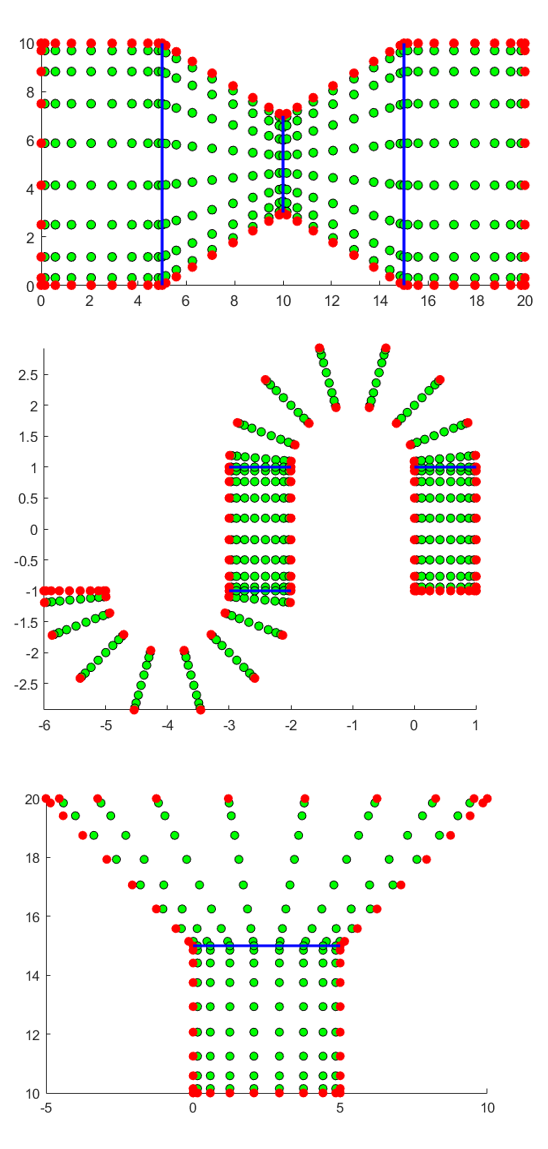
\includegraphics[width=3.4cm]{CurrentDisc.png}
			\end{figure}
		\column{0.5\linewidth}

    \begin{itemize}
    	\item Reduce both PDEs to systems of ODEs.
    	\item Discretize time (accurate interpolation).
    	\item Equations can now be solved using a DAE solver \\
    	(when given all necessary inputs).
    	\item For more 'complex' domains, pseudospectral methods are extended to spectral element methods.
    \end{itemize}


	\column{0.25 \linewidth}
	\vspace{-0.5cm}
	\begin{figure}
		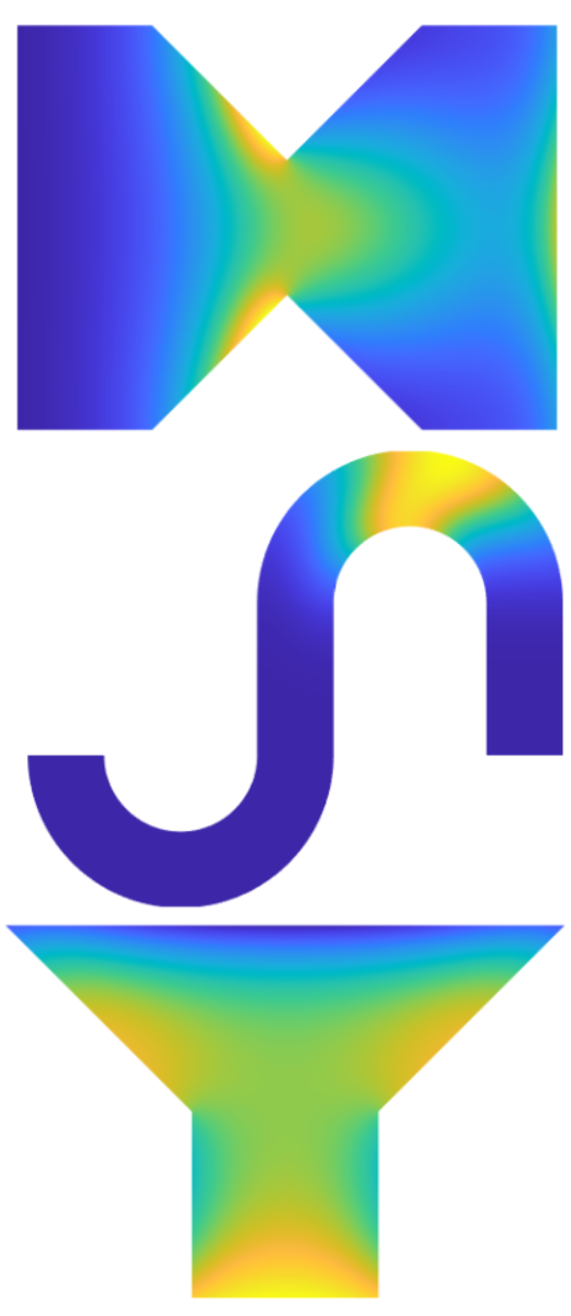
\includegraphics[width=3cm]{Current.png}
	\end{figure}
\end{columns}

\end{frame}


\begin{frame}
	\frametitle{Numerical Methods}
\framesubtitle{Fixed point algorithm}
\vspace{0.2 cm}
Initialize with guess $\textcolor{blue}{\vec{w}^{(0)}}$.
	\begin{enumerate}
     \item 
     Solve 
     	$ \displaystyle\partial_t \rho  = \nabla^2 \rho  - \nabla \cdot (\rho \textcolor{blue}{\vec{w}^{(i)}} ) + \nabla \cdot \left( \rho \nabla V_{\text{ext}} \right)
     	+ \nabla \cdot \int_\Omega \rho(\vec{x}) \rho(\vec{x}\hspace{0.2em}') \nabla V_2(|\vec{x}-\vec{x}\hspace{0.2em}'|)d\vec{x}\hspace{0.2em}'.$
	 \item
     Solve 
     	$\partial_{{\tau}} q  = \displaystyle \nabla^2 q  + \nabla q  \cdot \textcolor{blue}{\vec{w}^{(i)}} - \nabla q \cdot \nabla V_{\text{ext}} + \textcolor{ForestGreen}{\rho^{(i)}}  - \widehat \rho$\\
     	$\displaystyle \qquad \qquad \qquad \quad \ - \int_\Omega \textcolor{ForestGreen}{\rho^{(i)}(\vec{x}\hspace{0.2em}')} \bigg(\nabla q( \vec{x} ) - \nabla q( \vec{x}\hspace{0.2em}')\bigg) \cdot \nabla V_2(|\vec{x}-\vec{x}\hspace{0.2em}'|)d\vec{x}\hspace{0.2em}'. $
     \item Solve $\displaystyle \textcolor{blue}{\vec{w}^{(i)}_g} = - \frac{1}{\beta}\textcolor{ForestGreen}{{\rho}^{(i)}} \nabla \textcolor{red}{{q}^{(i)}}.$\\
     \item Measure the error: $ \mathcal{E} = ||\textcolor{blue}{\vec{w}^{(i)}} - \textcolor{blue}{\vec{w}^{(i)}_g}||$.
     \vspace{0.2 cm}
	 \item Update control, with $\lambda \in [0,1]$:       $\quad \textcolor{blue}{\vec{w}^{(i+1)}} = (1-\lambda)\textcolor{blue}{\vec{w}^{(i)}} + \lambda \textcolor{blue}{\vec{w}^{(i)}_g}.$	 
	\end{enumerate}	
\vspace{0.2 cm}
Iterate until $\mathcal{E} <TOL$.
\end{frame}

\begin{frame}
	\frametitle{Optimization for DDFT}
	\framesubtitle{Reminder: (Simple) DDFT model}
	\begin{align*}
		&\min_{\rho,\vec{w}} \quad \frac{1}{2}\norm{\rho- \widehat{\rho}}_{L_2(\Sigma)}^2 + \frac{\beta}{2} \norm{ {\vec{w}}}_{L_2(\Sigma)}^2\\
		\\
		&\text{subject to:}
		\\
		& \partial_t \rho = \nabla^2 \rho - \nabla \cdot (\rho  {\vec{w}}) + \nabla \cdot \left( \rho \nabla V_{\text{ext}} \right) + {\nabla \cdot \int_\Omega \rho(\vec{x}) \rho(\vec{x}\hspace{0.2em}') \nabla V_2(|\vec{x}-\vec{x}\hspace{0.2em}'|)d\vec{x}\hspace{0.2em}'} \qquad { \text{in    } \Sigma}\\
		\\
		&{\text{BC } \text{and IC:}}\\
		&\frac{\partial \rho}{\partial n} - \rho  {\vec{w}} \cdot \vec{n} + \rho \frac{\partial V_{\text{ext}}}{\partial n} + { \int_\Omega \rho(\vec{x}) \rho(\vec{x}\hspace{0.2em}')  \frac{ \partial  V_2}{\partial n}(|\vec{x}-\vec{x}\hspace{0.2em}'|)d\vec{x}\hspace{0.2em}'} {= 0 \qquad \quad \qquad \qquad \qquad \text{on   } \partial \Sigma  } \\
		&{\rho(0,\vec{x}) = \rho_0(\vec{x})} 
	\end{align*}
	
\end{frame}

\begin{frame}
	\frametitle{Results - Example 1}
	Overall Cost: $\mathcal J = \frac{1}{2}\norm{\rho- \widehat{\rho}}_{L_2(\Sigma)}^2 + \frac{\beta}{2} \norm{\vec{w}}_{L_2(\Sigma)}^2$, $\mathcal J_{\vec{w}= \vec 0} = 0.0400$.
    \vspace{0.3 cm}
	\begin{figure}
		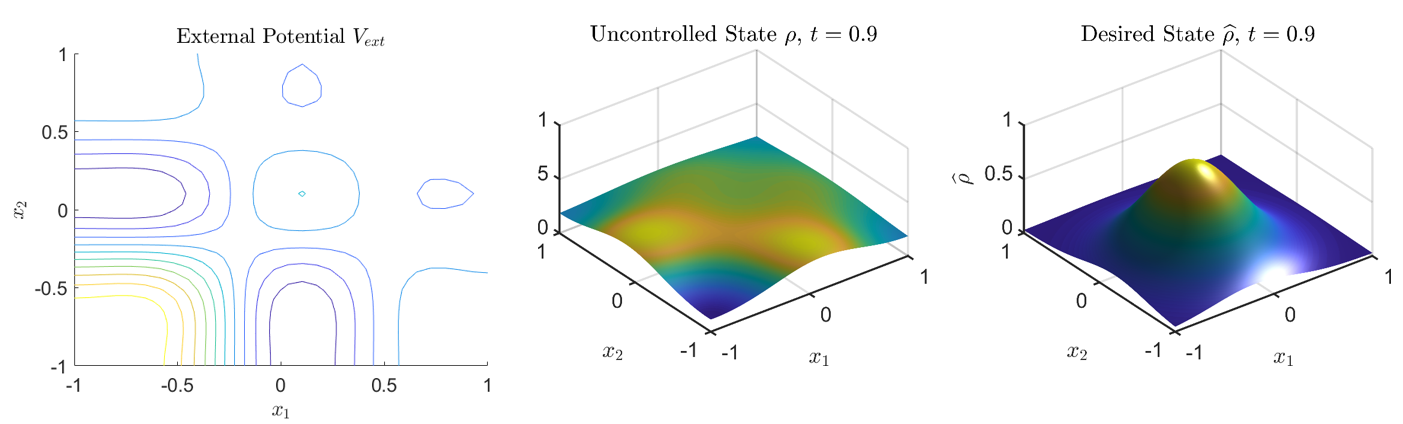
\includegraphics[width=14.5cm]{Figure32Db.png}
	\end{figure}
	
\end{frame}

\begin{frame}
	\frametitle{Results - Example 1}
	\vspace{0.3cm}
	Overall Cost: $\mathcal J = \frac{1}{2}\norm{\rho- \widehat{\rho}}_{L_2(\Sigma)}^2 + \frac{\beta}{2} \norm{\vec{w}}_{L_2(\Sigma)}^2$, $\mathcal J_{\vec{w} = \vec 0} = 0.0400$, $\mathcal J_{\text{opt}} = 0.0046$.
	\begin{figure}
		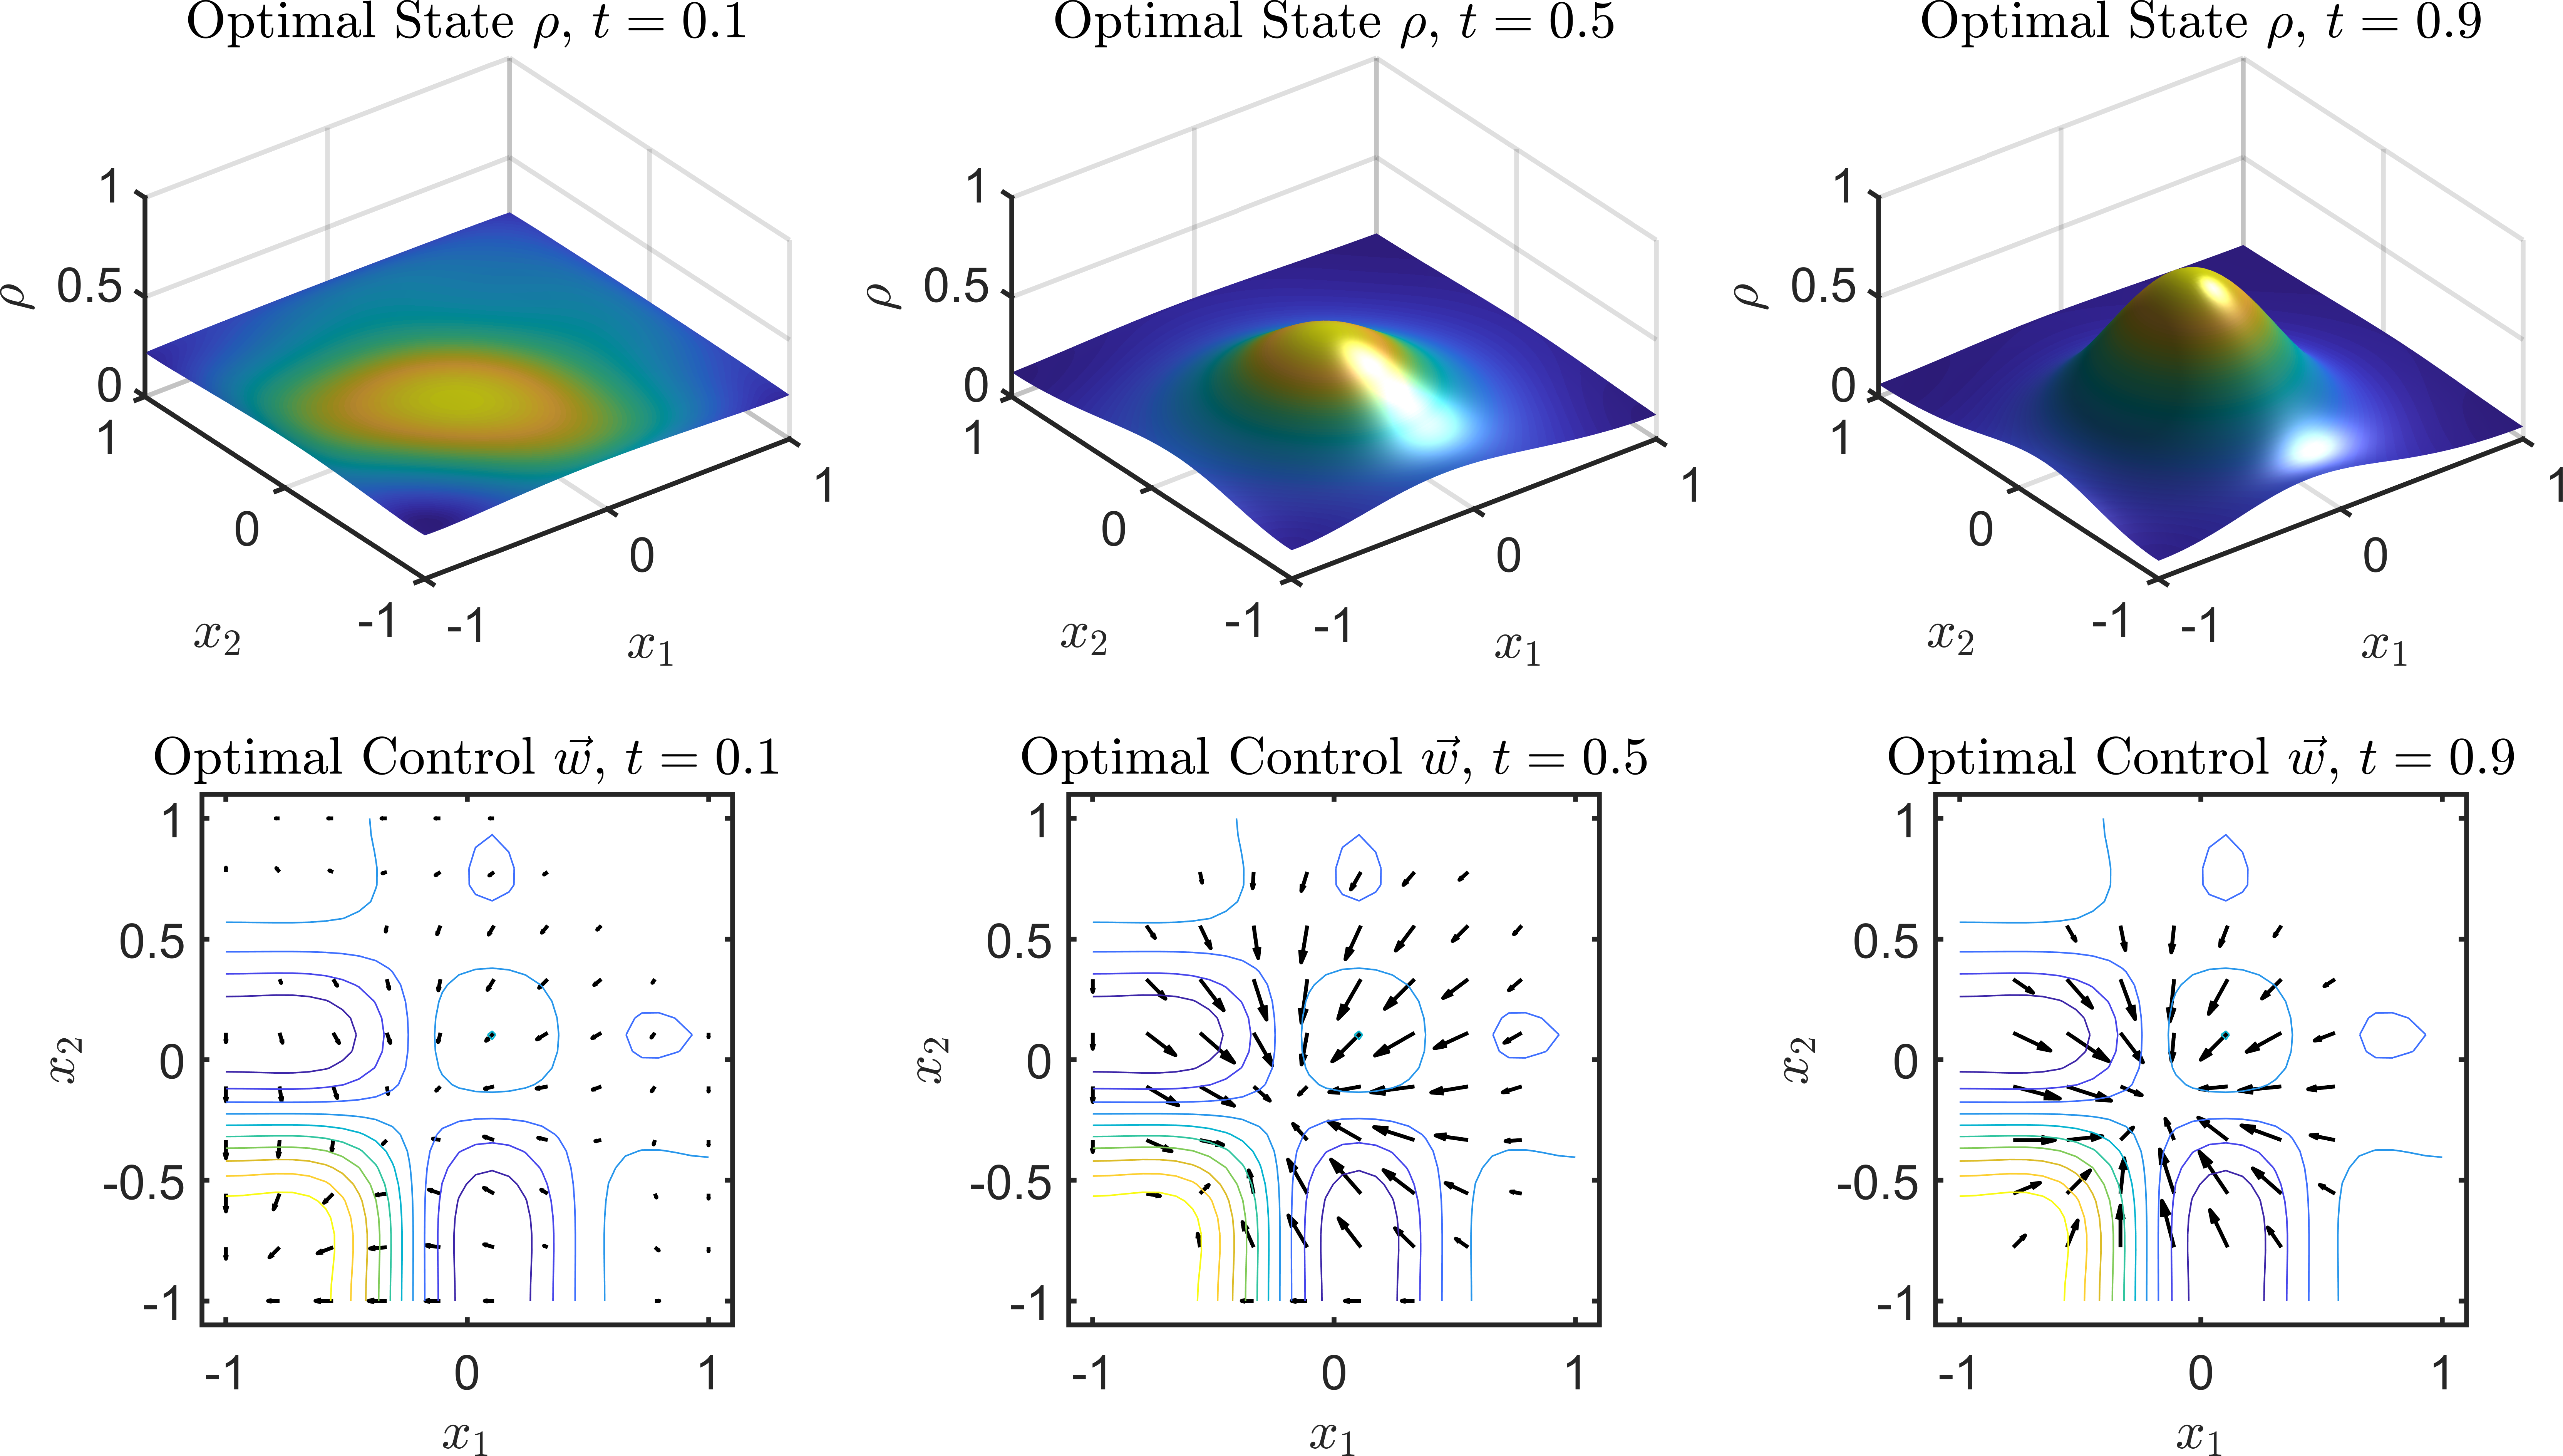
\includegraphics[width=12cm]{Figure42D.png}
	\end{figure}
\end{frame}

\begin{frame}
	\frametitle{Optimization for DDFT}
	\framesubtitle{A more general DDFT model}
	\begin{align*}
		&\min_{\rho,\vec{w}} \quad \frac{1}{2}\norm{\rho- \widehat{\rho}}_{L_2(\Sigma)}^2 + \frac{\beta}{2} \norm{ {\vec{w}}}_{L_2(\Sigma)}^2\\
		\\
		&\text{subject to:}
		\\
		& \ \partial_t \rho = \nabla \cdot \left( \rho \nabla \frac{\delta \textcolor{RoyalBlue}{ \mathcal F [\rho]} }{\delta \rho} - \rho  {\vec{w}}\right):= - \nabla \cdot \vec j \qquad \ \ { \text{in    } \Sigma}\qquad\qquad\qquad\qquad\\
		&\textcolor{RoyalBlue}{ \mathcal F [\rho]=  \mathcal F_{id}[\rho] + \mathcal F_{ext}[\rho] +  \mathcal F_{int}[\rho] + \int_\Omega \rho \left(-1 -\ln(1 - a\rho) + \frac{1}{1-a\rho}  \right)d \vec x} \\
		\\
		&{\text{BC } \text{and IC:}}\\
		&\vec j \cdot \vec n = 0 \quad \ \qquad \quad \qquad \qquad\qquad\qquad\qquad\qquad \text{on   } \partial \Sigma   \qquad\qquad\qquad\qquad\qquad \qquad \qquad\qquad \qquad \qquad\\
		&{\rho(0,\vec{x}) = \rho_0(\vec{x})} 
	\end{align*}
\end{frame}
\begin{frame}
	\frametitle{Results - Example 2}
	Overall Cost: $\mathcal J = \frac{1}{2}\norm{\rho- \widehat{\rho}}_{L_2(\Sigma)}^2 + \frac{\beta}{2} \norm{\vec{w}}_{L_2(\Sigma)}^2$, $\mathcal J_{\vec{w}= \vec 0} = 0.0484$.
	\vspace{0.3 cm}
	\begin{figure}
		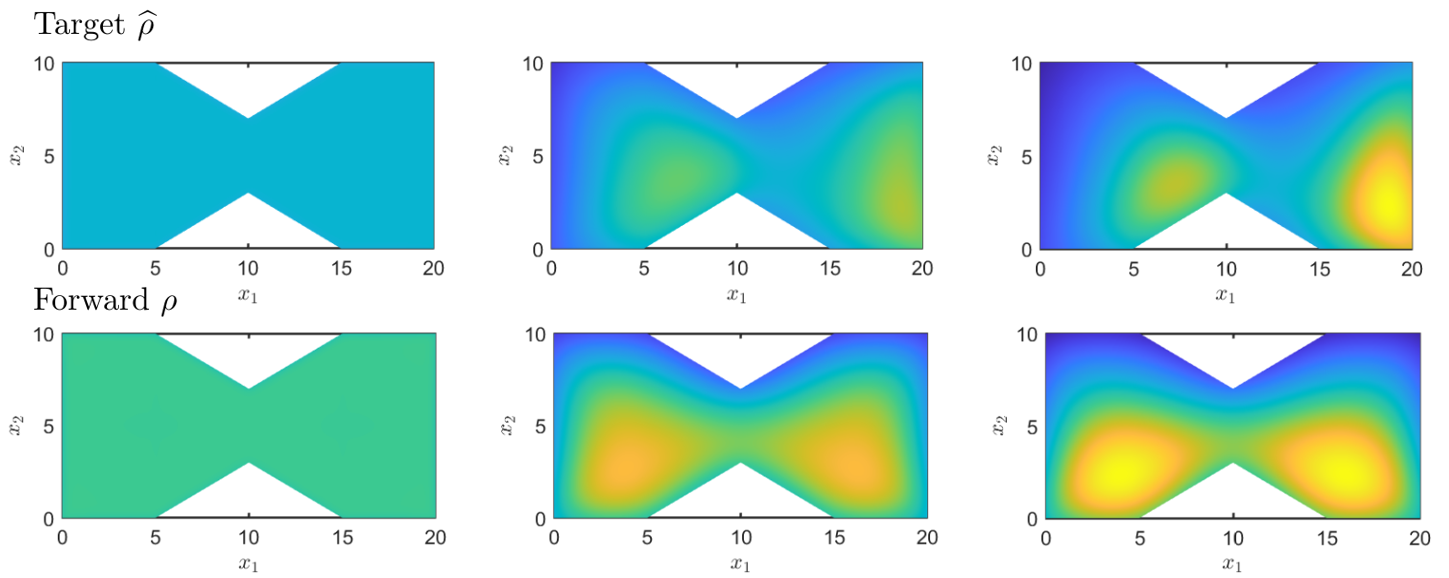
\includegraphics[width=14cm]{ExRes2a2.png}
	\end{figure}
	
\end{frame}
\begin{frame}
	\frametitle{Results - Example 2}
	\vspace{0.3cm}
	Overall Cost: $\mathcal J = \frac{1}{2}\norm{\rho- \widehat{\rho}}_{L_2(\Sigma)}^2 + \frac{\beta}{2} \norm{\vec{w}}_{L_2(\Sigma)}^2$, $\mathcal J_{\vec{w} = \vec 0} = 0.0484$, $\mathcal J_{\text{opt}} = 0.0146$.
	\begin{figure}
		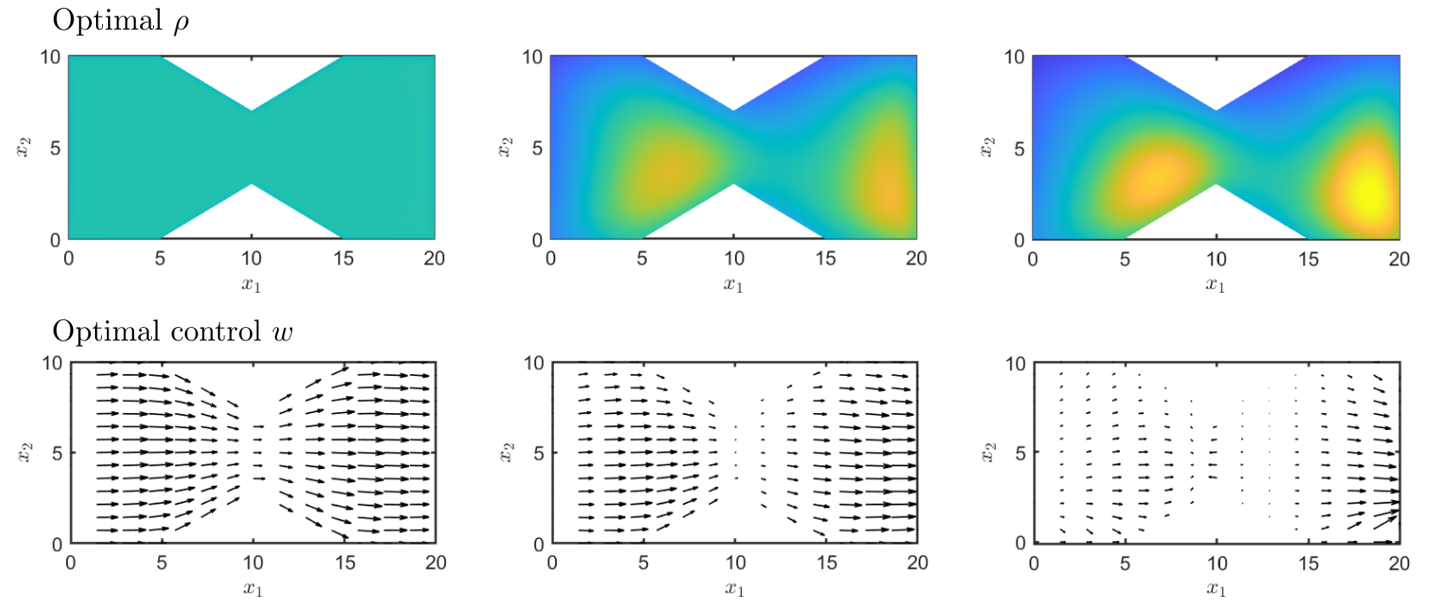
\includegraphics[width=14cm]{ExRes2b3.png}
	\end{figure}
\end{frame}




\begin{frame}
	\frametitle{Summary}
	\begin{columns}
		\column{0.2 \linewidth}
		\vspace{-0.5cm}
		\begin{figure}
			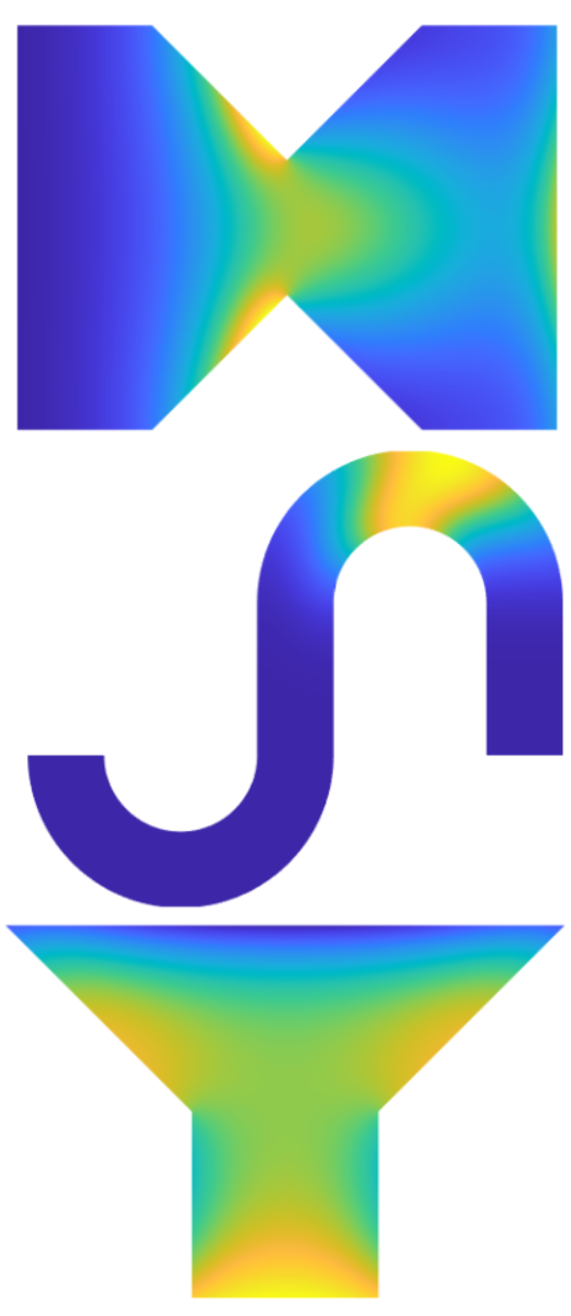
\includegraphics[width=3.2cm]{Current.png}
		\end{figure}
		
		
	\column{0.6 \linewidth}
	Up to now:
	\begin{itemize}
		\item Deriving PDE-constrained optimization models.
		\item Developing a suitable numerical method to solve them.
	\end{itemize}
	Current:
	\begin{itemize}
		\item Complex domains.
		\item Extended PDE models.
		\item Different boundary conditions.
	\end{itemize}
	Up next:
	\begin{itemize}
		\item More extended models.
		\item Different controls.
		\item Application to industrial processes.
	\end{itemize}
	\column{0.2 \linewidth}
	\vspace{-0.6cm}
	\begin{figure}
		
\includegraphics[width=2.7cm]{west.png}\\
		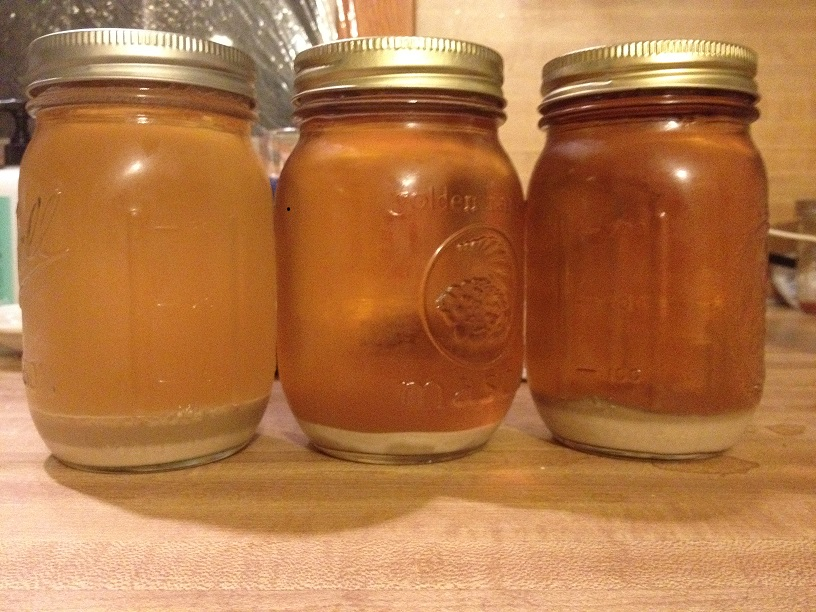
\includegraphics[width=3cm]{beer.png}\\
		
\includegraphics[width=3cm]{ufraction8.png}\\
		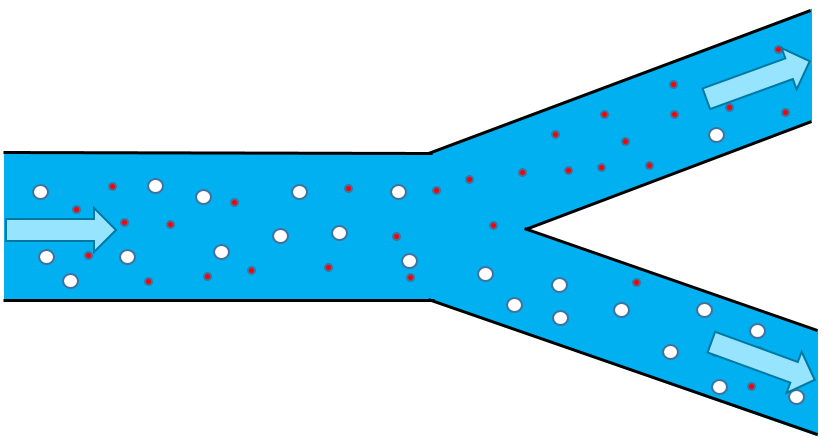
\includegraphics[width=3cm]{Microfilter.png}
	\end{figure}
	\end{columns}
\end{frame}

\appendix




\begin{frame}
\frametitle{Some References}    
\begin{thebibliography}{10}    

	\bibitem{Us2020}
	M. Aduamoah, B. D. Goddard, J. W. Pearson and J. C. Roden.
	\newblock {\em PDE-constrained optimization models and pseudospectral methods for multiscale particle dynamics.} 
	\newblock { \em Preprint, 2020.}
	
	\bibitem{Archer1}
	A. J.   Archer  and  A.  Malijevský . 
	\newblock {\em On the interplay between sedimentation and phase separation phenomena in two-dimensional colloidal fluids.}
	\newblock { \em Molecular Physics,} 109, 1087-1099, 2011. 
	
	\bibitem{Autor1990}
	A. Nold, B.D. Goddard, P. Yatsyshin, N. Savva and S. Kalliadasis. 
	\newblock {\em 	Pseudospectral methods for density functional theory in bounded and unbounded domains}.
	\newblock {\em Journal of Computational Physics}, 334, 639-664, 2017.
	\newblock \url{https://datashare.is.ed.ac.uk/handle/10283/2647} (2DChebClass)
		
\end{thebibliography}
\end{frame}
\begin{frame}
\frametitle{Some More References}    
\begin{thebibliography}{10}    
	
	
	\bibitem{Burger1}
	M. Burger, M. Di Francesco, P.A. Markowich and  M.-T. Wolfram. 
	\newblock {\em Mean field games with nonlinear mobilities in pedestrian dynamics.}
	\newblock { \em Discrete and Continuous Dynamical Systems - Series B,} 19(5), 1311-1333, 2014. 	

	
\end{thebibliography}
\end{frame}


\begin{frame}
	\frametitle{Results - Example 2, with Time-Independent Control}
	\vspace{0.3cm}
	Overall Cost: $\mathcal J = \frac{1}{2}\norm{\rho- \widehat{\rho}}_{L_2(\Sigma)}^2 + \frac{\beta}{2} \norm{\vec{w}}_{L_2(\Omega)}^2$, $\mathcal J_{\vec{w} = \vec 0} = 0.0484$, $\mathcal J_{\text{opt}} = 0.0258$.
	\begin{figure}
		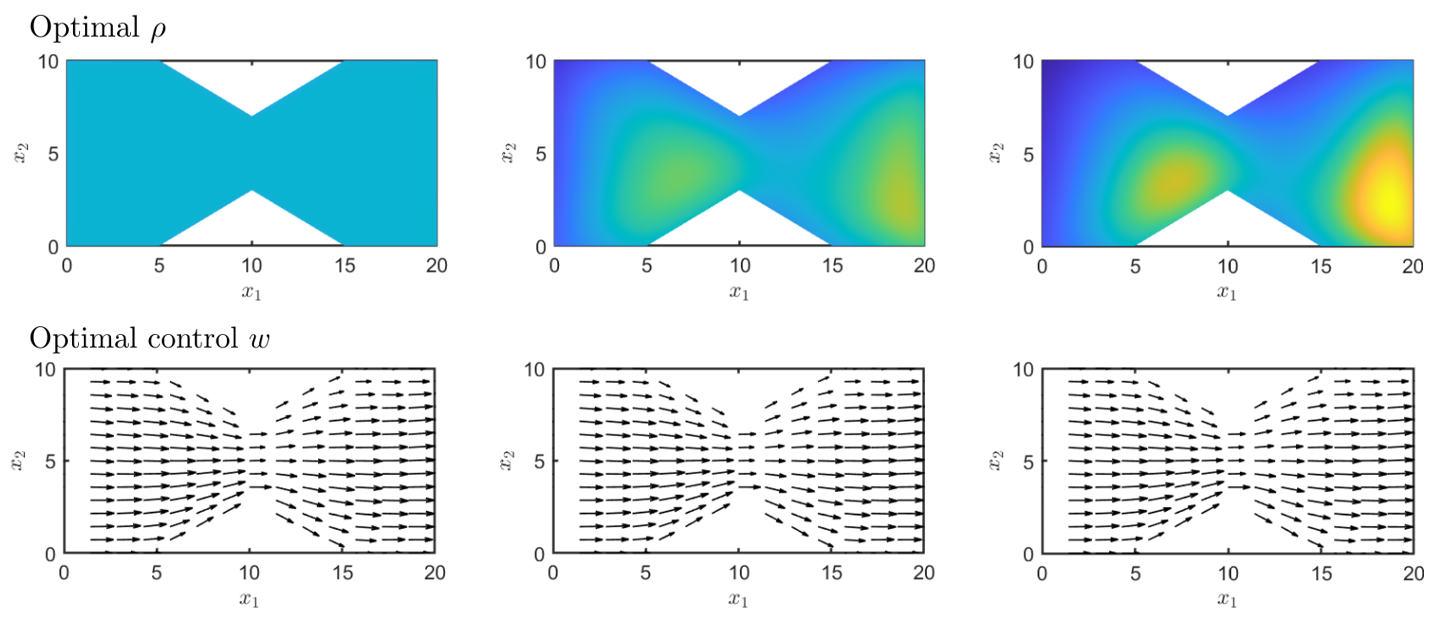
\includegraphics[width=14cm]{ExRes2b2.png}
	\end{figure}
\end{frame}




\begin{frame}
	\frametitle{Data for Example 1}
	\begin{table}
		\centering
		\begin{tabular}{ | c | c || c | c | c | c ||}
			\hline
			\multicolumn{2}{|c||}{}& $\beta = 10^{-3}$ & $\beta = 10^{-1}$ & $\beta = 10^{1}$ & $\beta = 10^{3}$  \\
			\hline
			\hline
			& $\mathcal J_{\vec{w} = \vec 0}$ & $\numprint{0.0400}$ & $\numprint{0.0400}$ & $\numprint{0.0400}$ & $\numprint{0.0400}$ \\
			$\kappa= \numprint{-1}$  & $\mathcal{J}_{\text{opt}}$ & $\numprint{0.0046}$ & $\numprint{0.0370}$ & $\numprint{0.0400}$ & $\numprint{0.0400}$ \\
			& \texttt{Iter} & $\numprint{717}$ & $\numprint{778}$ & $\numprint{347}$ & $\numprint{1}$ \\
			\hline
			& $\mathcal J_{\vec{w} = \vec 0}$ & $\numprint{0.0478}$ & $\numprint{0.0478}$ & $\numprint{0.0478}$ & $\numprint{0.0478}$ \\
			$\kappa= \numprint{0}$  & $\mathcal{J}_{\text{opt}}$ & $\numprint{0.0064}$ & $\numprint{0.0450}$ & $\numprint{0.0478}$ & $\numprint{0.0478}$ \\
			& \texttt{Iter} & $\numprint{718}$ & $\numprint{784}$ & $\numprint{343}$ & $\numprint{1}$ \\
			\hline
			& $\mathcal J_{\vec{w} = \vec 0}$ & $\numprint{0.0556}$ & $\numprint{0.0556}$ & $\numprint{0.0556}$ & $\numprint{0.0556}$ \\
			$\kappa= \numprint{1}$  & $\mathcal{J}_{\text{opt}}$ & $\numprint{0.0085}$ & $\numprint{0.0530}$ & $\numprint{0.0556}$ & $\numprint{0.0556}$ \\
			& \texttt{Iter} & $\numprint{720}$ & $\numprint{787}$ & $\numprint{339}$ & $\numprint{1}$ \\
			\hline
		\end{tabular}
		\caption{Cost when $\vec{w}=\vec{0}$, optimal control cost, and iterations required, for a range of values for interaction strength $\kappa$ and regularization parameter $\beta$.}
		\label{TabS5:Prob22D}
	\end{table}
\end{frame}


\begin{frame}
	\frametitle{References: Figures}   
	\begin{thebibliography}{10}    
		\bibitem{F1}
		ufraction8 Logo. Digital Image. \newblock{ \em www.ufraction8.}
		\url{ufraction8.com}
		
		\bibitem{F2}
		WEST Logo. Digital Image. \newblock{\em WEST Brewery} \url{www.westbeer.com}
	\end{thebibliography}	
\end{frame}




\end{document}